\documentclass{amsart}

\usepackage[french]{babel}
\usepackage{graphicx}

\newtheorem{theorem}{Théorème}[section]
\newtheorem{lemma}[theorem]{Lemme}

\theoremstyle{definition}
\newtheorem{definition}[theorem]{Définition}
\newtheorem{example}[theorem]{Exemple}
\newtheorem{xca}[theorem]{Exercice}

\theoremstyle{remark}
\newtheorem{remark}[theorem]{Remarque}

\numberwithin{equation}{section}

%    Absolute value notation
\newcommand{\abs}[1]{\lvert#1\rvert}

%    Blank box placeholder for figures (to avoid requiring any
%    particular graphics capabilities for printing this document).
\newcommand{\blankbox}[2]{%
  \parbox{\columnwidth}{\centering
%    Set fboxsep to 0 so that the actual size of the box will match the
%    given measurements more closely.
    \setlength{\fboxsep}{0pt}%
    \fbox{\raisebox{0pt}[#2]{\hspace{#1}}}%
  }%
}

\renewcommand*{\overrightarrow}[1]{\vbox{\halign{##\cr 
  \tiny\rightarrowfill\cr\noalign{\nointerlineskip\vskip1pt} 
  $#1\mskip2mu$\cr}}}

\begin{document}

\title{Électron libre}

\author{Bellevue (BLV)}

\begin{abstract}
    Cet article contient la résolution de nombreuses questions du problème \og Électron libre \fg{} de la quatorzième édition du Tournoi Français
    des Jeunes Mathématiciennes et Mathématiciens. La résolution de problème est composé de lemmes, théorèmes et conjectures énoncés à la suite.
\end{abstract}

\maketitle

\tableofcontents

\section{Introduction}

Nicolas joue dispose d’un canon à électrons immergé dans un champ magnétique constant uniforme. À l'aide de son canon, il peut émettre un électron 
circulant alors à vitesse constante en décrivant un cercle dans le sens trigonométrique, que l'on a supposé de rayon 1. 

Il dispose aussi d’un bouton qui permet de faire faire demi-tour à l’électron tel qu'au moment où il appuie, la vitesse de l’électron reste la même 
mais progresse dans la direction opposée.

Le coeur du problème réside dans l'optimisation entre la longueur totale de la courbe de la trajectoire, du nombre d'appuies, ainsi que la restriction 
de la taille de la trajectoire selon l'espace.\newpage
\section{Définitions}

\begin{definition}
  On appelle \textbf{trajet} une courbe permettant de relier deux points A,B dans un plan quelconque. Voici des exemples de trajets:

  \begin{figure}[!h]
    \centering
    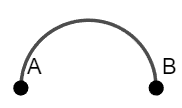
\includegraphics[scale=0.5]{circle.png}
    \caption{Un trajet circulaire.}
  \end{figure}

  \begin{figure}[!h]
    \centering
    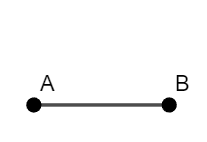
\includegraphics[scale=0.5]{line.png}
    \caption{Un trajet étant le segment [AB].}
  \end{figure}

  \begin{figure}[!h]
    \centering
    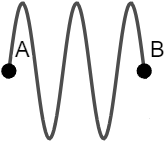
\includegraphics[scale=0.5]{sinus.png}
    \caption{Un trajet sinusoïdal.}
  \end{figure}
\end{definition}

\begin{definition}
  On appelle $\lambda(A,B)$ la longueur d'une courbe dans un plan quelconque reliant deux points A,B. Dans le cadre de la courbe d'une fonction $f$,
  on considère donc que: \[\lambda(A,B)=\int_{x_a}^{x_b} \sqrt{1+{f^\prime}^2} \,dx\]
  
  (La démonstration est effectuée à la suite de l'article).
\end{definition}

\begin{definition}
  On appelle $n_{bouton}$ le nombre de fois que l'on appuie sur le bouton permettant de changer le sens trigonométrique de la trajectoire.
\end{definition}

\begin{definition}
  On appelle \textbf{distance absolue} la plus petite distance séparant deux points A,B dans un plan quelconque, soit le segment [AB]. On la note $d_{abs}$. (Voir le \textbf{Théorème 4.1}.)
\end{definition}

\begin{definition}
  On appelle un \textbf{demi-cercle trigonométrique perpétuel} une courbe composée de plusieurs addition d'$1/2$ circonférence d'un cercle trigonométrique (soit $\pi$). Voici une illustration ci-dessous:

  \begin{figure}[!h]
    \centering
    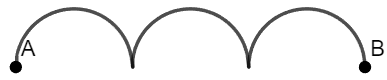
\includegraphics[scale=0.5]{demicircle.png}
    \caption{Un demi-cercle trigonométrique perpétuel répété 3 fois.}
  \end{figure}
\end{definition}

\section{Lemmes}

\begin{lemma}
  Soit $a,b\in\mathbb{R}$. Soit $f,g$ deux fonctions $\in\mathbb{R}$. Si $f(x)\le g(x) \implies$

  \[\int_{a}^{b}f(x) \,dx \le \int_{a}^{b}g(x) \,dx\]
\end{lemma}

\section{Théorèmes utilitaires}

\begin{theorem}
  Soit $f$ une fonction. Soit $a,b\in\mathbb{R}$. On considère la longueur de la courbe de $f$ allant de $a$ à $b$ étant égale à:
  
  \[\lambda(a,b)=\int_{a}^{b} \sqrt{1+{f^\prime}^2} \,dx\]
\end{theorem}

\begin{proof}
  
\end{proof}

\begin{theorem}
  Soit A,B deux points dans un plan quelconque. On admet que le trajet le plus court afin d'aller de A à B est une ligne droite.
\end{theorem}

\begin{proof}
  Considérons deux points A,B dans un plan quelconque. Soit le repère orthonormé (A;I;J) tel que \overrightarrow{AJ} $\perp$ \overrightarrow{AB}. On considère donc les points A($x_a=0,y_a=0$) et B($x_b,y_b=0$).
  
  Soit $f_q, f_q\in\mathbb{R}$, une fonction continue sur $[x_a,x_b]$ modélisant le trajet de A à B (n'étant pas une droite, avec $f_q(x)=0$ à $x_a$ et $x_b$, pour compléter la courbe). Soit $f_k$, une fonction
  continue sur $[x_a,x_b]$, $f_k\in\mathbb{R}$, modélisant la droite entre A et B, donc $f_k(x)=0$.
  
  En effectuant un raisonnement par l'absurde, supposons que $\exists f_q,f_q\in\mathbb{R},f_q(x_a)=f_q(x_b)=0$ mais non $f_q(x)=0, \forall x\in\mathbb{R}$, tel que $\lambda_q(A,B) < \lambda_k(A,B)$.

  $0$ étant une constante, on sait que $f_k^\prime(x)=0$:

  \[\implies \lambda_k(A,B)=\int_{x_a}^{x_b}1 \,dx \iff \lambda_k(A,B)= x_b-x_a \]

  Or $f_q(x)\ne 0,\forall x\in\mathbb{R} \implies f_q(x)$ doit avoir une valeur dépendant de $x$ (et non pas juste d'une constante $k$ ou $kx, k\in\mathbb{R}$, car dans un tel cas, $f_q(x_a)\ne f_q(x_b)$). 

  \[\implies \lambda_q(A,B)=\int_{x_a}^{x_b}\sqrt{1+f_q{^\prime}(x)^2} \,dx\]

  Nous savons donc que: 

  \[1 < \sqrt{1+f_q{^\prime}(x)^2}\] 
  
  $\forall x \in \mathbb{R}$ car $f_q{^\prime}(x)^2> 0, \forall x \in \mathbb{R}$, avec la fonction racine carré étant croissante sur $\mathbb{R}$:

  \[\implies \int_{x_a}^{x_b}1 \,dx < \int_{x_a}^{x_b}\sqrt{1+f_q{^\prime}(x)^2} \,dx\] 
  
  (D'après la \textbf{Lemme 3.1}).

  On en déduit que $\lambda_k(A,B) < \lambda_q(A,B)$, soit le trajet le plus court pour aller de A à B étant une ligne droite.
\end{proof}

\begin{theorem}
  La plus grande distance possible sur la courbe d'un cercle est sa circonférence divisée par 2 (le diamètre).
\end{theorem}

\begin{theorem}
  Soit A,B deux points dans un plan orthonormé. Avec un trajet formant un demi-cercle trigonométrique perpétuel de A à B et la possibilité de changer de direction à des points $C_0, C_1$, ... $C_{n-1}, C_{n}$ (selon l'énoncé),$n\in\mathbb{N}$, le trajet le plus court
  est le demi-cercle trigonométrique perpétuel de A à B.
\end{theorem}

\begin{proof}
  On comprend qu'avec le \textbf{Théorème 4.2}, afin de maximiser la distance minimale entre A et B, il faut trouver un moyen de telle sorte que la courbe partant de A et allant à B aie une forme semblable à une droite. 
  Le problème réside donc dans la question: Il y a t'il un moyen de conformer les points A, C et B afin de faire une courbe se rapprochant d'une droite.
\end{proof}

\section{Question 1.1}

\begin{theorem}
  Soit A,B deux points dans un plan quelconque. Il est toujours possible d'atteindre B en partant de A en formant des demi-cercles trigonométrique perpétuels et en pouvant choisir l'orientation initiale.
\end{theorem}

\begin{proof}
  On considère un point A dans un plan quelconque et $C_a$, le cercle trigonométrique passant par A.

  À $n_{bouton}=0$, pouvant choisir l'orientation de base du cercle trigonométrique, on en déduit que l'on peut former un nouveau cercle $C_{a^\prime}$ selon les possibilités d'orientation.  $C_{a^\prime}$ a donc pour rayon $r_{a^\prime}\in\mathbb{R^+}, r_{a^\prime}=2$, étant le 
  diamètre du cercle trigonométrique. Cela couvre donc tous les points ayant une distance $d=2$ de A, soit donc une surface de $4\pi$.

  Après avoir parcouru une trajectoire $T=\pi$. D'après le \textbf{Théorème 4.3}, on considère le fait d'appuyer sur le bouton ($n_{bouton}=1$) pour pouvoir progresser dans le plan. Par le même raisonnement que lorsque $n_{bouton}=0$,
  on en déduit que l'on peut former un nouveau cercle $C_{a^{\prime\prime}}$ selon les possibilités d'orientation.  $C_{a^{\prime\prime}}$ a donc pour rayon $r_{a^{\prime\prime}},=2r_{a^\prime}=4$ et une surface de $16\pi$.

  Par récurrence, on déduit que l'on peut toujours former un cercle $C_k$ de rayon $r_k=2(n_{bouton}+1) \implies$ lorsque $n_{bouton}\to+\infty$, $r_k\to+\infty \implies {\pi}r_k^2\to+\infty$, couvrant ainsi l'ensemble du plan.

  On comprend donc qu'il est possible à partir du point A d'atteindre n'importe quel point B dans le plan.


  Voici une représentation visuelle permettant d'expliquer le raisonnement:
  \begin{figure}[!h]
    \centering
    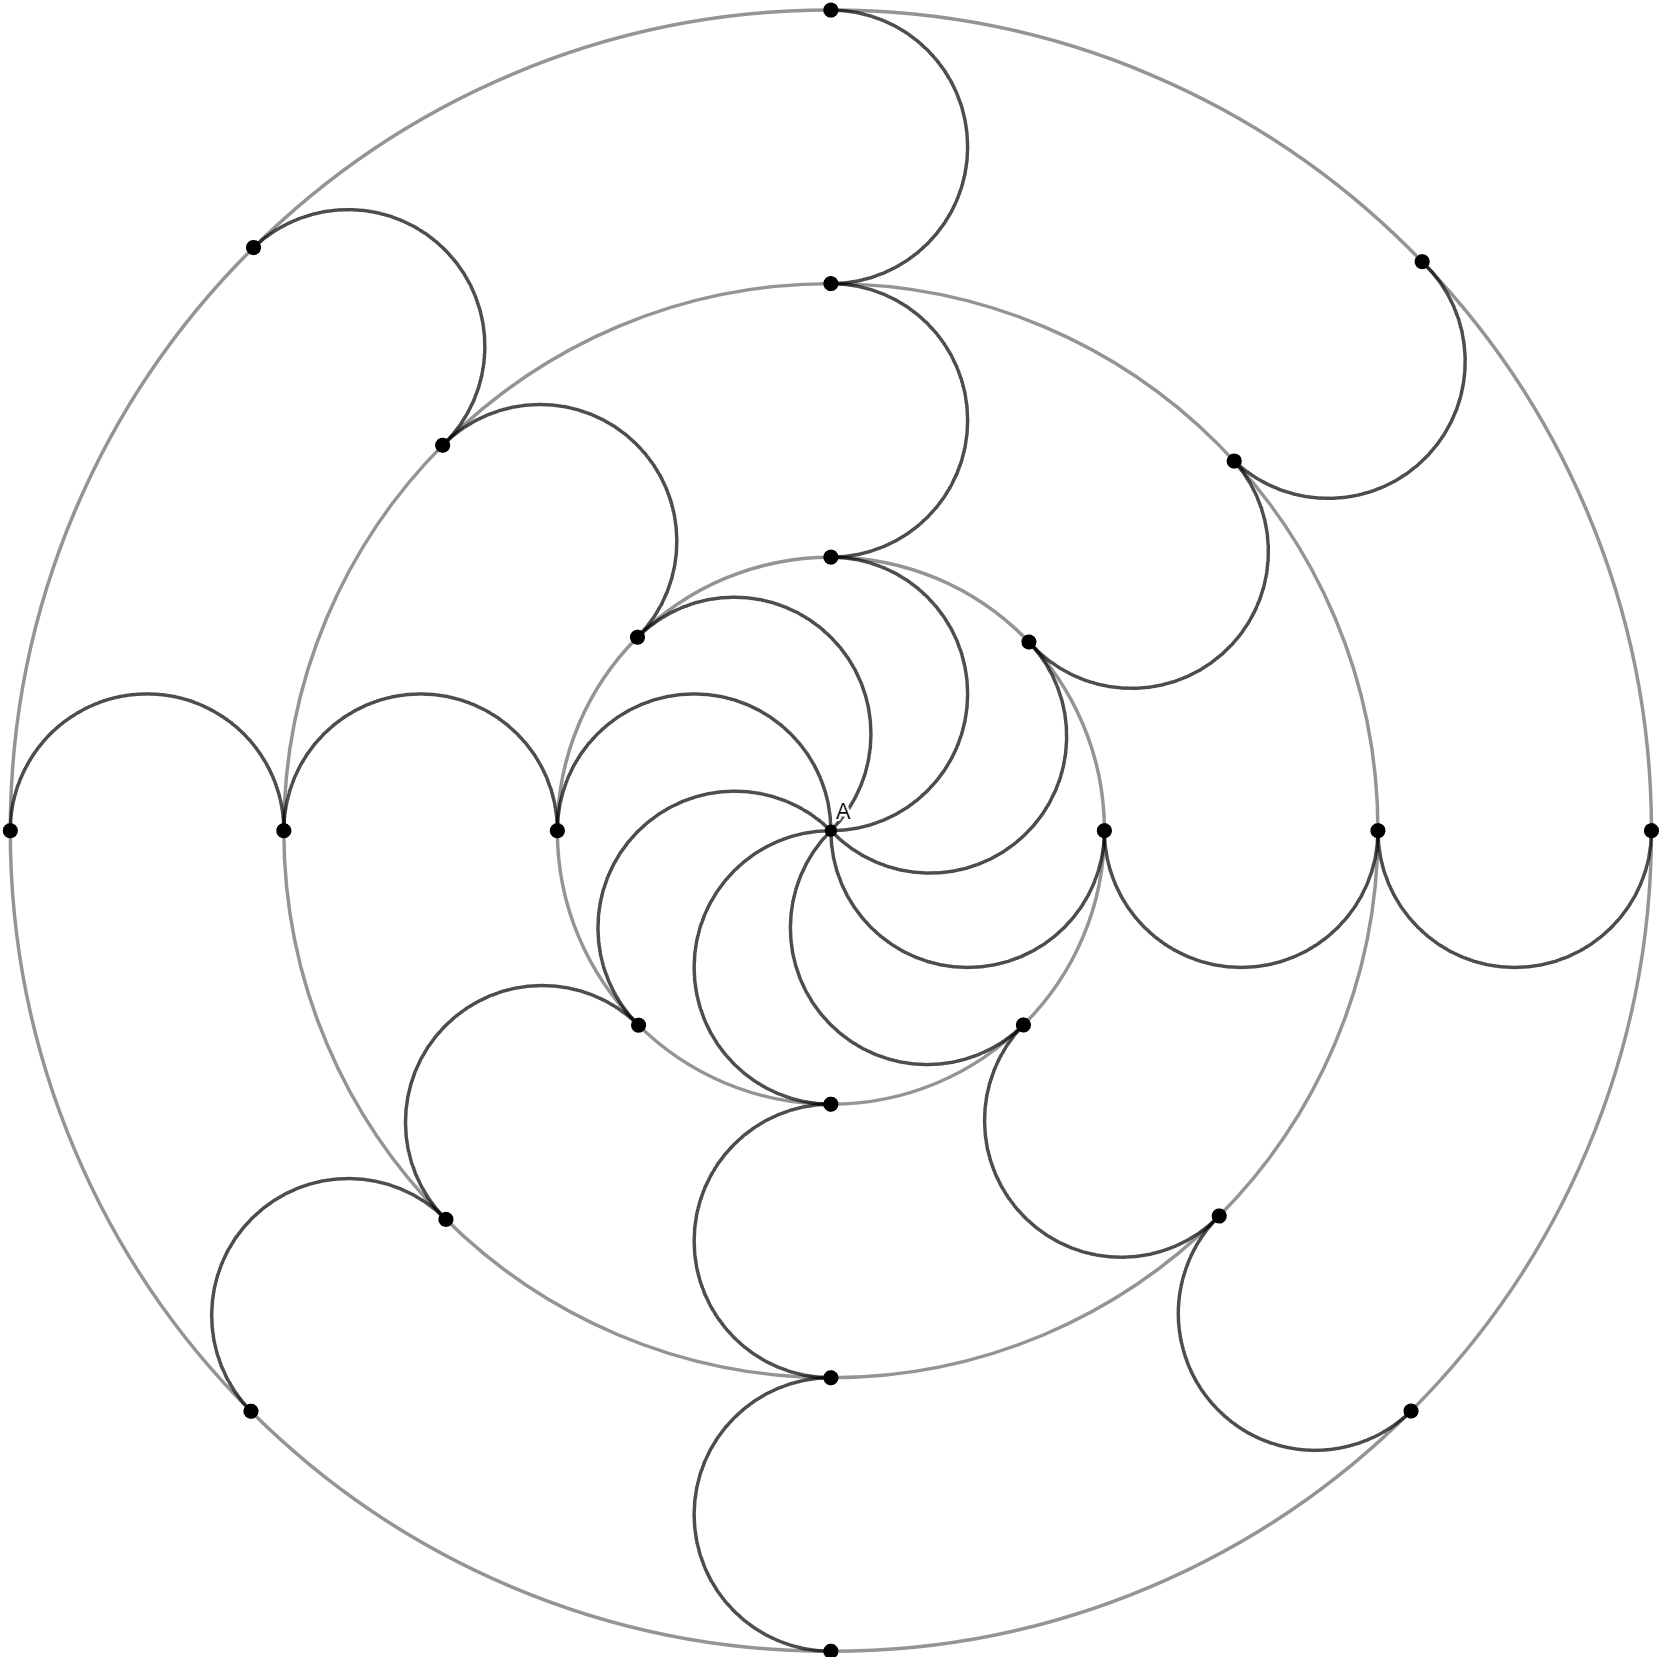
\includegraphics[scale=0.27]{visualization.png}
    \caption{Représentations des moyens d'atteindre B en partant de A avec une division=8 selon l'orientation (les points des courbes circulaires ont donc un angle de 45° entre eux selon le point A) avec $n_{bouton}=2$. 
    Les points noirs sont des points B avec la longueur du segment [AB] un multiple de $\pi$.}
  \end{figure}
\end{proof}

\end{document}